% 20 / 02 /2009 v1.00c TKZdoc-tab-tv
\section{Création d'un tableau de variations : \addbs{tkzTab}}
\subsection{Définition} 
\begin{NewMacroBox}{tkzTab}%
{\oarg{local options}\var{liste1}\var{liste2}\var{liste3}\var{liste4}}

\medskip
\begin{tabular}{lllc}
\hline
\texttt{arguments}   & \texttt{défaut}    & \texttt{définition}                 \\
\hline
\IargName{tkzTab}{liste1}  & |no default|  & \var{e(1)/h(1),\dots,e(p)/h(p)} première colonne     \\
\IargName{tkzTab}{liste2}  & |no default|  & \var{a(1),\dots,a(n)}    antécédents de la première ligne  \\
\IargName{tkzTab}{liste3}  & |no default|  & \var{s(1),\dots,s(2n-1)} symboles de la ligne de signes   \\
\IargName{tkzTab}{liste4}  & |no default|  & \var{s(1)/eg(1)/ed(1),\dots,s($q$)/eg($q$)/ed($q$)} variations     \\
\hline
\end{tabular}

\medskip
\noindent\emph{La macro \emph{\tkzcname{tkzTab}} est un raccourci pour enchaîner \tkzcname{tkzTabInit}, \tkzcname{tkzTabLine}  et \tkzcname{tkzTabVar}. Les \tkzname{options} sont identiques à celles de \tkzcname{tkzTabInit}. Ces tableaux ne concernent que les tableaux à trois lignes pour la variable, le signe de la dérivée et les variations de la fonction.}
\end{NewMacroBox}

\medskip

\begin{tkzexample}[code only]
 \tkzTab{ e(1) / h(1) ,
             ... ,
          e(p) / h(p)}
        { v(1), ... ,v(n) }
        { a(1),...,a(2n-1)}
        { s(1) / eg(1) / ed(1), ... ,s(n) / eg(n) / ed(n)}
\end{tkzexample}

\subsection{Exemple 1} 

Étude de la fonction $f~:~ x \longmapsto x^2$ sur $[-5~;~7]$

\begin{tkzexample}[vbox,very small]
\begin{tikzpicture}
\tkzTab[lgt=3,espcl=5]{ $x$                    / 1,
                        $f'(x)$                / 1,
                        Variations de \\$f$ / 2}
                      { $-5$ , $0$ ,$7$}
                      { ,-,z,+,}
                      { +/$25$  , -/$0$  , +/ $49$}%
\end{tikzpicture}\end{tkzexample}

\subsection{Exemple 2} 
Étude de la fonction $f~:~ x \longmapsto x \ln x $ sur $]0~;~+\infty]$

\begin{tkzexample}[vbox,very small]
 \begin{tikzpicture}
 \tkzTab[espcl=5,lgt=3]{$x$ / 1, Signe de \\$\ln x +1$ / 1.5,%
   Variations de \\$f$ / 3}%
   {$0$ ,$1/\E$ , $+\infty$}{d,-,z,+,}
   {D+/ $0$,%
    -/ \colorbox{black}{\textcolor{white}{$\dfrac{-1}{e}$}}  ,%
    +/ $+\infty$ }%
\end{tikzpicture}\end{tkzexample}

\subsection{Exemple 3} 
 Étude de  la fonction $f~:~ $x$ \longmapsto \sqrt{x^2-1}$ sur $]-\infty~;~-1] \cup [1~;~+\infty[$
 
\begin{tkzexample}[vbox,very small]
\begin{tikzpicture}
  \tkzTab{ $x$ / 1, $f'(x)$ / 1, $f$ / 2}%
         { $-\infty$, $-1$ ,$1$, $+\infty$}
         { ,-,d,h,d,+, }
         { +/$+\infty$  , -H/$0$, -/$0$  , +/ $+\infty$  }%
\end{tikzpicture}\end{tkzexample}

\subsection{Exemple 4} 
 Étude de  la fonction $f~:~ $t$ \longmapsto \frac{t^2}{t^2-1}$ sur $[0~;~+\infty[$
 
\begin{tkzexample}[vbox,very small]
\begin{tikzpicture}
  \tkzTab{ $t$ / 1, Signe de\\ $f'(t)$ / 2, Variation de \\$f$ / 2}%
         { $0$, $1$, $+\infty$}
         { z , - , d , - , }
         { +/$0$  , -D+/$-\infty$/$+\infty$, -/ $1$  }%
\end{tikzpicture}\end{tkzexample}
\endinput

